\section{Polynomial Hierarchy, Alternating TMs}

\begin{figure}
\centering
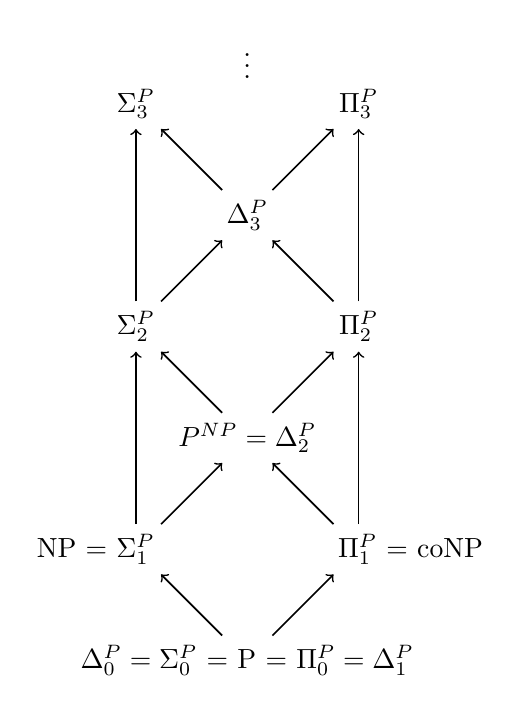
\begin{tikzpicture}[->, node distance=2cm, semithick]
 \node (P) {$\Delta_0^\text{P} =\Sigma_0^\text{P}$ = P = $\Pi_0^\text{P} = \Delta_1^\text{P}$};
 \node (Sigma1) [above left of=P]       {NP = $\Sigma_1^\text{P}$ \hspace*{0.9cm}};
 \node (Pi1)    [above right of=P]      {\hspace*{1.2cm} $\Pi_1^\text{P}$ = coNP};
 \node (Delta2) [above left of=Pi1]     {$\text{P}^\text{NP} = \Delta_2^\text{P}$};
 \node (Sigma2) [above left of=Delta2]  {$\Sigma_2^\text{P}$};
 \node (Pi2)    [above right of=Delta2] {$\Pi_2^\text{P}$};
 \node (Delta3) [above left of=Pi2]     {$\Delta_3^\text{P}$};
 \node (Sigma3) [above left of=Delta3]  {$\Sigma_3^\text{P}$};
 \node (Pi3)    [above right of=Delta3] {$\Pi_3^\text{P}$};
 \node (dots)   [above of=Delta3]       {\vdots};
 \draw (P)      -> (Sigma1);
 \draw (P)      -> (Pi1);
 \draw (Sigma1) -> (Sigma2);
 \draw (Sigma1) -> (Delta2);
 \draw (Pi1)    -> (Pi2);
 \draw (Pi1)    -> (Delta2);
 \draw (Delta2) -> (Sigma2);
 \draw (Delta2) -> (Pi2);
 \draw (Sigma2) -> (Sigma3);
 \draw (Sigma2) -> (Delta3);
 \draw (Pi2)    -> (Pi3);
 \draw (Pi2)    -> (Delta3);
 \draw (Delta3) -> (Sigma3);
 \draw (Delta3) -> (Pi3);
\end{tikzpicture}
\caption{Polynomial Hierarchy, taken from http://commons.wikimedia.org/wiki/File:Polynomial\_time\_hierarchy.svg}
\end{figure}